\section{The MPC Problem}

The Optimal Control Problem to be solved was chosen in such a way as to make
analysis of the models' performances more straightforward. The objective is
tracking a defined reference temperature as close as possible, while ensuring
the heat input stays within the HVAC capacity. The \textit{zero-variance} method
is used for multi-step prediction when using an existing \acrshort{gp}. This
does ignore the propagation of uncertainty for multi step ahead prediction, but
even with its simplicity, this method has been proven to work
~\cite{kocijanModellingControlDynamic2016,jainLearningControlUsing2018,
pleweSupervisoryModelPredictive2020}.

The optimization problem is therefore defined as follows:

\begin{subequations}\label{eq:optimal_control_problem}
    \begin{align}
        & \text{minimize}
        & & \sum_{i=0}^{N-1} (\bar{y}_{t+i} - y_{ref, t})^2 \\
        & \text{subject to}
        & & \bar{y}_{t+i} = K_*K^{-1}\mathbf{x}_{t+i-1} \\
        &&& \mathbf{x}_{t+i-1} = \left[\mathbf{w}_{t+i-1},\quad
        \mathbf{u}_{t+i-1},\quad \mathbf{y}_{t+i-1}\right]^T \\
        \label{eq:components}
        &&& u_{t+i} \in \mathcal{U}
    \end{align}
\end{subequations}

where $y_{ref, t}$ is the reference temperature at time t, $\mathbf{x}_{t}$ is
the GP input vector at time t, composed of the exogenous autoregressive inputs
$\mathbf{w}_{t}$, the autoregressive controlled inputs $\mathbf{u}_{t}$ and the
autoregressive outputs $\mathbf{y}_{t}$.

\subsection{Temperature reference}

The temperature reference for the controller has been taken as the mean value of
the SIA~180:2014~\cite{sia180:2014ProtectionThermiqueProtection2014} temperature
norm. It imposes a range of temperatures that are allowed for residential
buildings based on the rolling 48h average outside temperature.


\begin{figure}[ht]
    \centering
    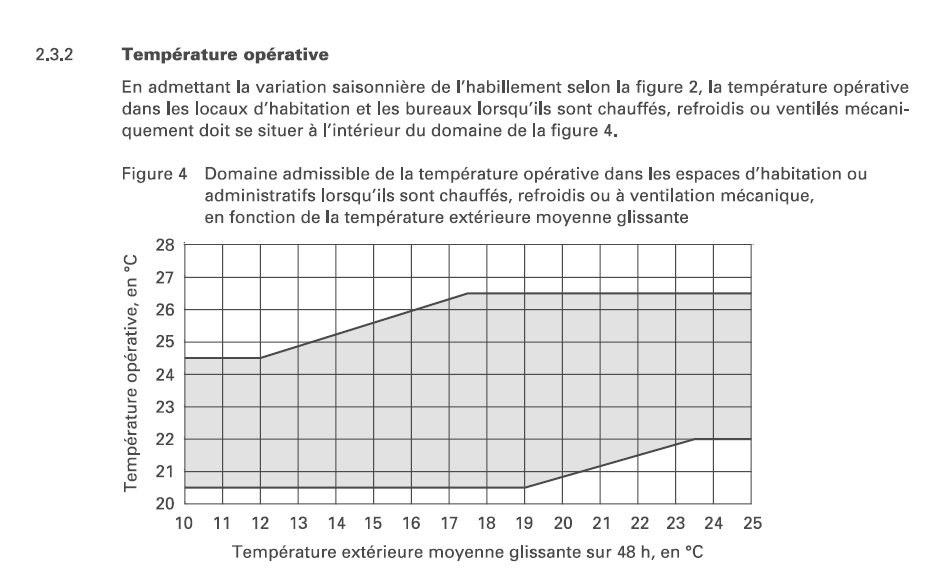
\includegraphics[width = \textwidth]{Images/sia_180_2014.png}
    \caption{The SIA 180:2014 norm for residential building temperatures}
    \label{fig:sia_temperature_norm}
\end{figure}

\clearpage
